\documentclass[tikz=true]{standalone}
%\usepackage{tikz}
\usepackage{tikzdefs}
\usepackage{amsfonts}
\begin{document}
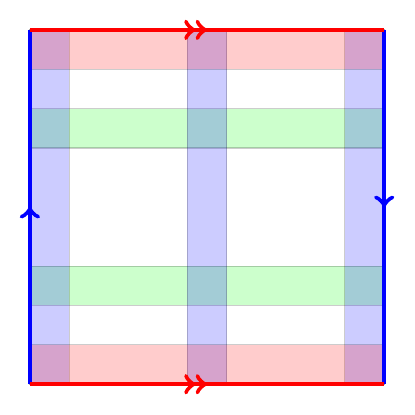
\begin{tikzpicture}[scale=0.5]
	\def\maxtheta{360}
	\def\maxphi{180}
	\def\rad{0.35}
	\def\offs{0.5}
	\def\idlen{2.0}

	% primary circle shade
	\filldraw[fill=green, opacity=0.2]
		(-\offs,1.5) rectangle (8+\offs,2.5);
	\filldraw[fill=green, opacity=0.2]
		(-\offs,5.5) rectangle (8+\offs,6.5);
	% secondary circle shade
		\filldraw[fill=blue, opacity=0.2]
		(-\offs,-\offs) rectangle (0.5,8+\offs);
	\filldraw[fill=blue, opacity=0.2]
		(7+\offs,-\offs) rectangle (8.5,8+\offs);
	\filldraw[fill=blue, opacity=0.2]
		(3.5,-\offs) rectangle (4.5,8+\offs);
	% even circle shade
	\filldraw[fill=red, opacity=0.2]
		(-\offs,-0.5) rectangle (8+\offs,0.5);
	\filldraw[fill=red, opacity=0.2]
		(-\offs,7.5) rectangle (8+\offs,8.5);

	\foreach \phi in {0,22.5,...,\maxphi} {
		\begin{scope}[shift={(\phi/\maxphi*8,0)}]
			\begin{scope}[shift={(0,0)}]
				\patchB{\rad}{\phi}
			\end{scope}
			\begin{scope}[shift={(0,1)}]
				\patchF{\rad}{\phi+180.0}
			\end{scope}
			\begin{scope}[shift={(0,2)}]
				\patchD{\rad}{\phi+180.0}
			\end{scope}
			\begin{scope}[shift={(0,3)}]
				\patchE{\rad}{\phi+180.0}
			\end{scope}
			\begin{scope}[shift={(0,4)}]
				\patchC{\rad}{\phi}
			\end{scope}
			\begin{scope}[shift={(0,5)}]
				\patchE{\rad}{\phi}
			\end{scope}
			\begin{scope}[shift={(0,6)}]
				\patchD{\rad}{\phi}
			\end{scope}
			\begin{scope}[shift={(0,7)}]
				\patchF{\rad}{\phi}
			\end{scope}
			\begin{scope}[shift={(0,8)}]
				\patchB{\rad}{\phi}
			\end{scope}
		\end{scope}
	}
	% left line
	\draw [blue,ultra thick] (-\offs,-\offs) -- (-\offs,8+\offs);
	\draw [->,blue,ultra thick] (-\offs,-\offs) -- (-\offs,4);
	% right line
	\draw [blue,ultra thick] (8+\offs,8+\offs) -- (8+\offs,-\offs);
	\draw [->,blue,ultra thick] (8+\offs,8+\offs) -- (8+\offs,4);
	% bottom line
	\draw [red,ultra thick] (-\offs,-\offs) -- (8+\offs,-\offs);
	\draw [->>,red,ultra thick] (-\offs,-\offs) -- (4,-\offs);
	% top line
	\draw [red,ultra thick] (8+\offs,8+\offs) -- (-\offs,8+\offs);
	\draw [->>,red,ultra thick] (-\offs,8+\offs) -- (4,8+\offs);


\end{tikzpicture}
\end{document}
